\documentclass[preprint2]{aastex}
\usepackage{natbib}
\usepackage{color}
\usepackage{booktabs}
\bibliographystyle{apj}

\shorttitle{Bright Point Size}
\shortauthors{Farris}

\begin{document}

\title{Determining coronal bright point size via cross-correlation using
multi-wavelength images from AIA/\textit{SDO}}
\author{Laurel Farris, R. T. James McAteer}
\affil{New Mexico State University}
\email{laurel07@nmsu.edu}

\begin{abstract}
\end{abstract}
\keywords{Sun: corona{-}Sun: bright points{-}}

\section{Introduction}\label{intro}

Bright points are located in the junctions between supergranules in the solar
photosphere. These are thought to be a result of magnetic flux tubes moving to
these junctions after rising to the surface and being jostled about by
advection (source: class notes?). Though they only cover about 1.6 \% of the
visible surface (\cite{Srivastava}), bright points (together with sunspots)
contribute over 90\% of the total magnetic flux (\cite{Howard}).

Over the course of the solar cycle, they can contribute significantly to the
global intensity variation of the sun, particularly in the ultraviolet
regime (\cite{Riethmuller}). UV flux from bright points can be studied using
their coronal counterparts.

These bright points can be seen in the upper layers of the solar atmosphere in
the form of coronal bright points. The cross-sectional area of these BPs is
known to increase in height as the density decreases and temperature increases
(source).


\section{Data}\label{data}
This analysis was carried out on data from AIA/\textit{SDO} (\cite{Lemen}).
A grayscale image of the full disk at the start of the time series () is shown
in figure %\ref{}.
A single coronal bright point was located and analyzed in each passband, of
which there were seven total. Each of these wavelengths corresponds to emission
from a different ion, hence a different temperature/height above the solar
photosphere.
An image of the bright point in each of the wavelengths is shown in figure
%\ref{},
also at the beginning of the time series.

The relevant values for each passband are given in table \ref{aia}.
\begin{table}[h]
\centering
    \begin{tabular}{c c c}
        \hline\hline
        Wavelength [\AA{}] & Temperature [K] & Height [km]\\
        \hline
        94 & $10^{6}$ & 11\\
        131 & $10^{6}$ & 11\\
        171 & $10^{6}$ & 11\\
        193 & $10^{6}$ & 11\\
        211 & $10^{6}$ & 11\\
        304 & $10^{6}$ & 11\\
        335 & $10^{6}$ & 11\\
        1600 & $10^{6}$ & 11\\
        1700 & $10^{6}$ & 11\\
        4500 & $10^{6}$ & 11\\
    \end{tabular}
\caption{stuff}
\label{aia}
\end{table}

\begin{figure*}[htb!]
    %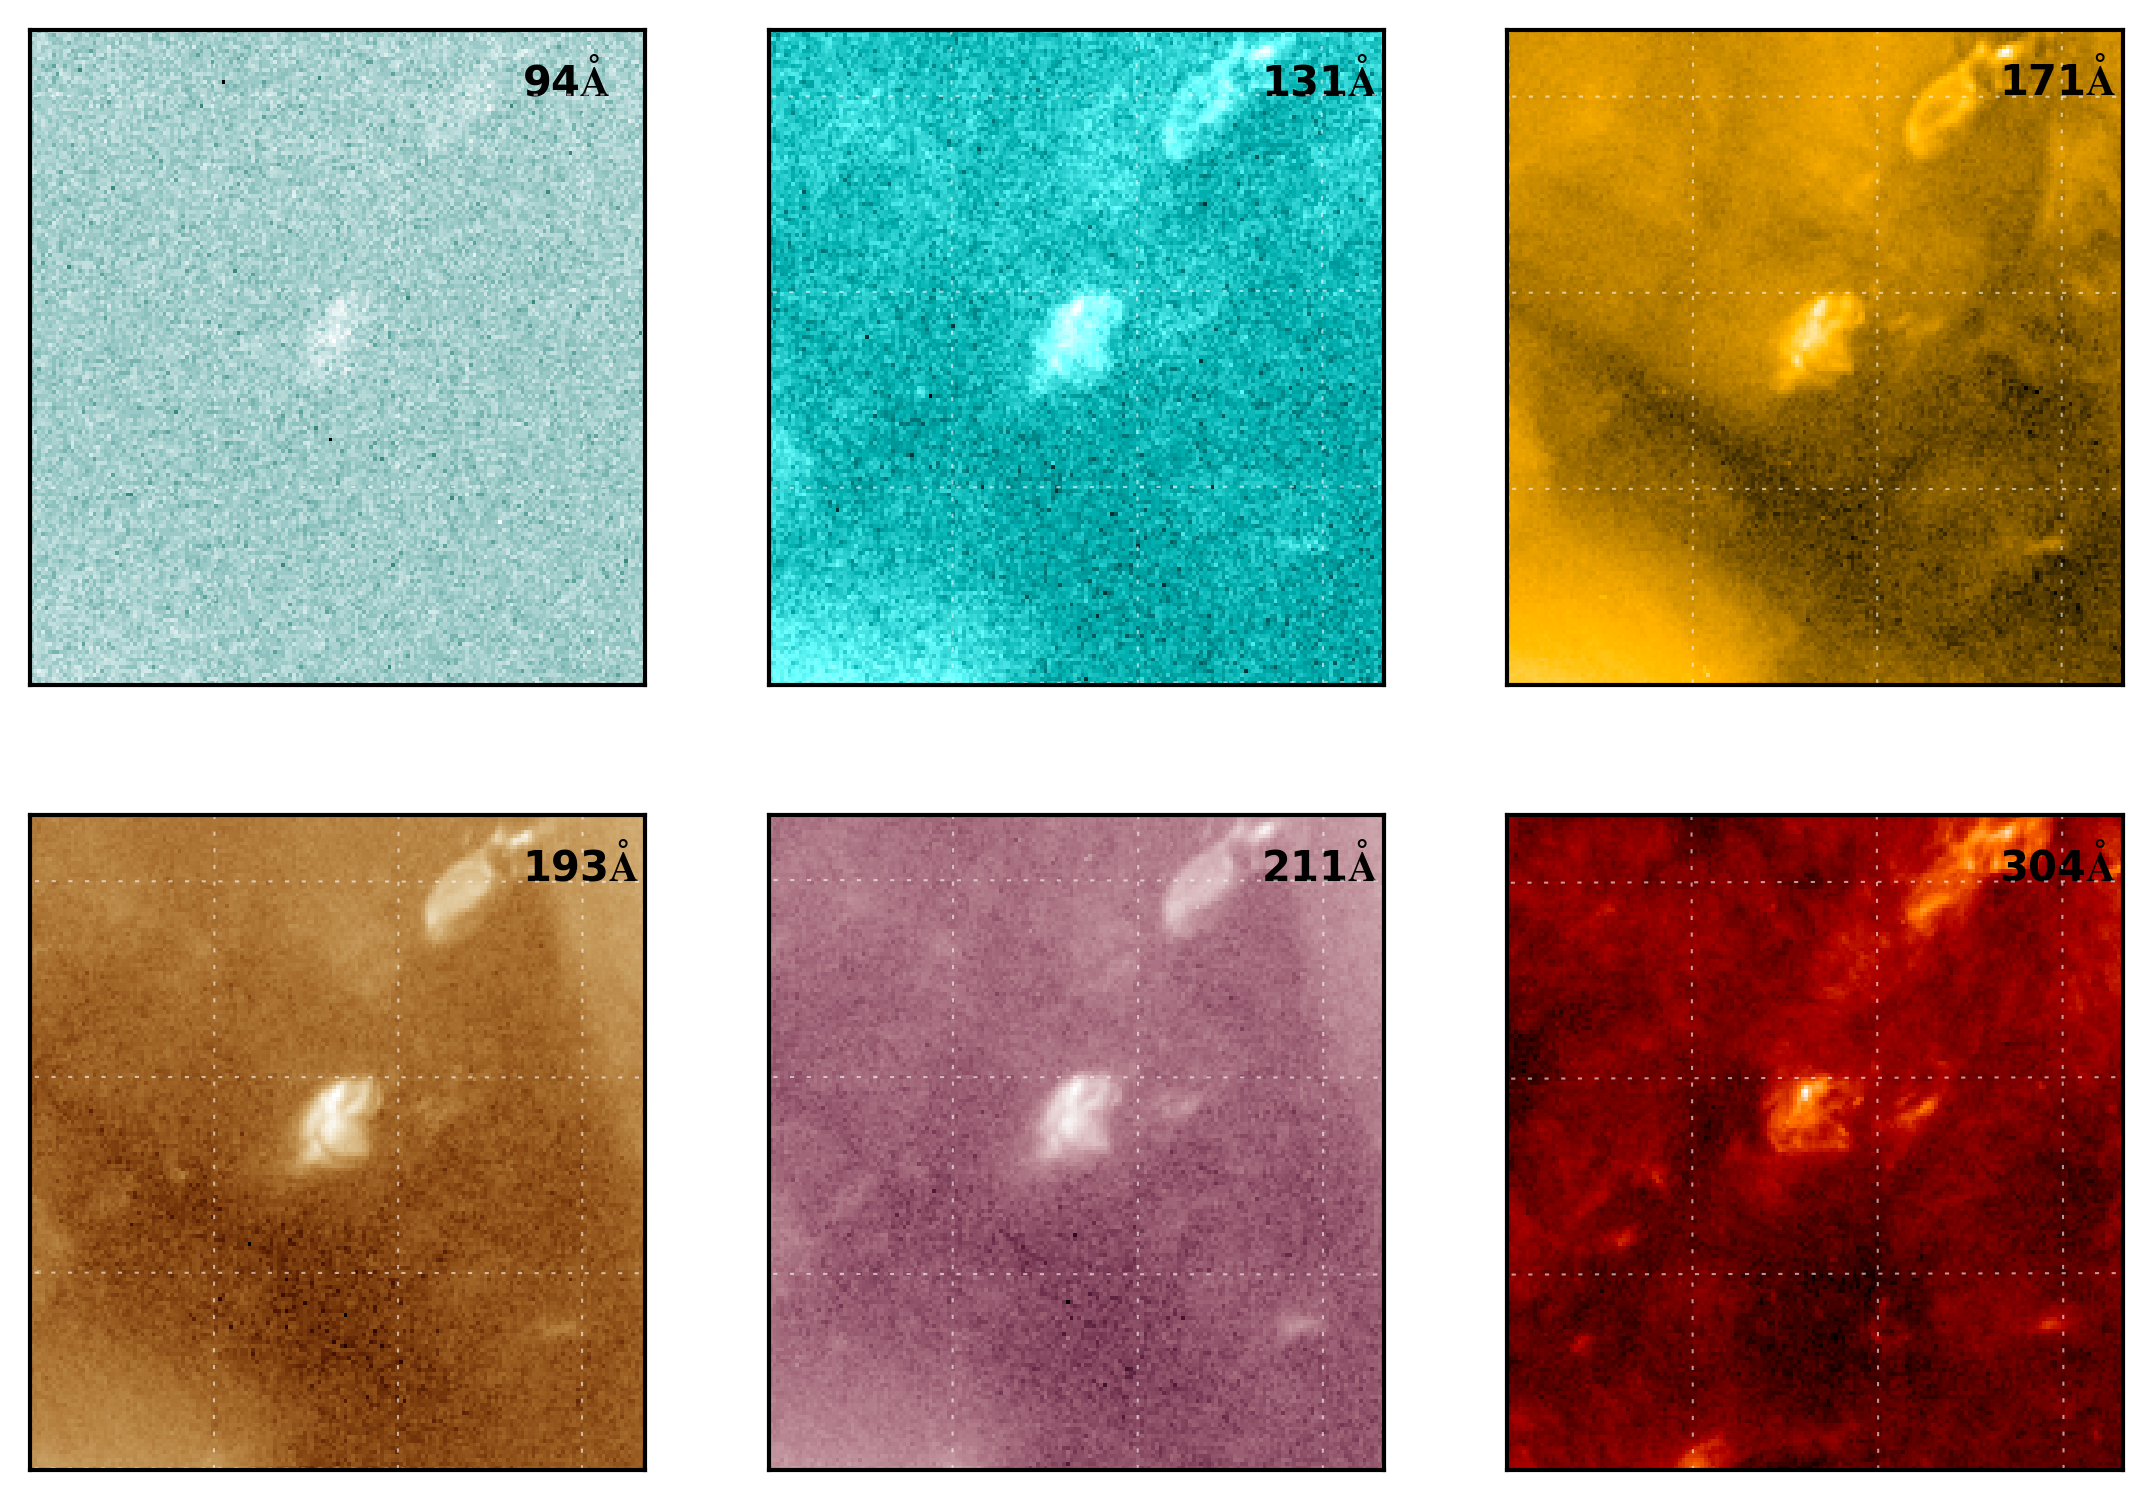
\includegraphics[width=\textwidth]{/solarstorm/laurel07/Research_repo/new_python_codes/bp_size/full_bp.png}
    \includegraphics[width=\textwidth]{images.png}
    \caption{Images of the BP in six different AIA wavelengths.}
\end{figure*}

\begin{figure*}[htb!]
    \includegraphics[width=\textwidth]{cc.png}
    \caption{Cross-correlation}
\end{figure*}

\begin{figure*}[htb!]
    \includegraphics[width=\textwidth]{tt.png}
    \caption{Timelag}
\end{figure*}

\begin{figure*}[htb!]
    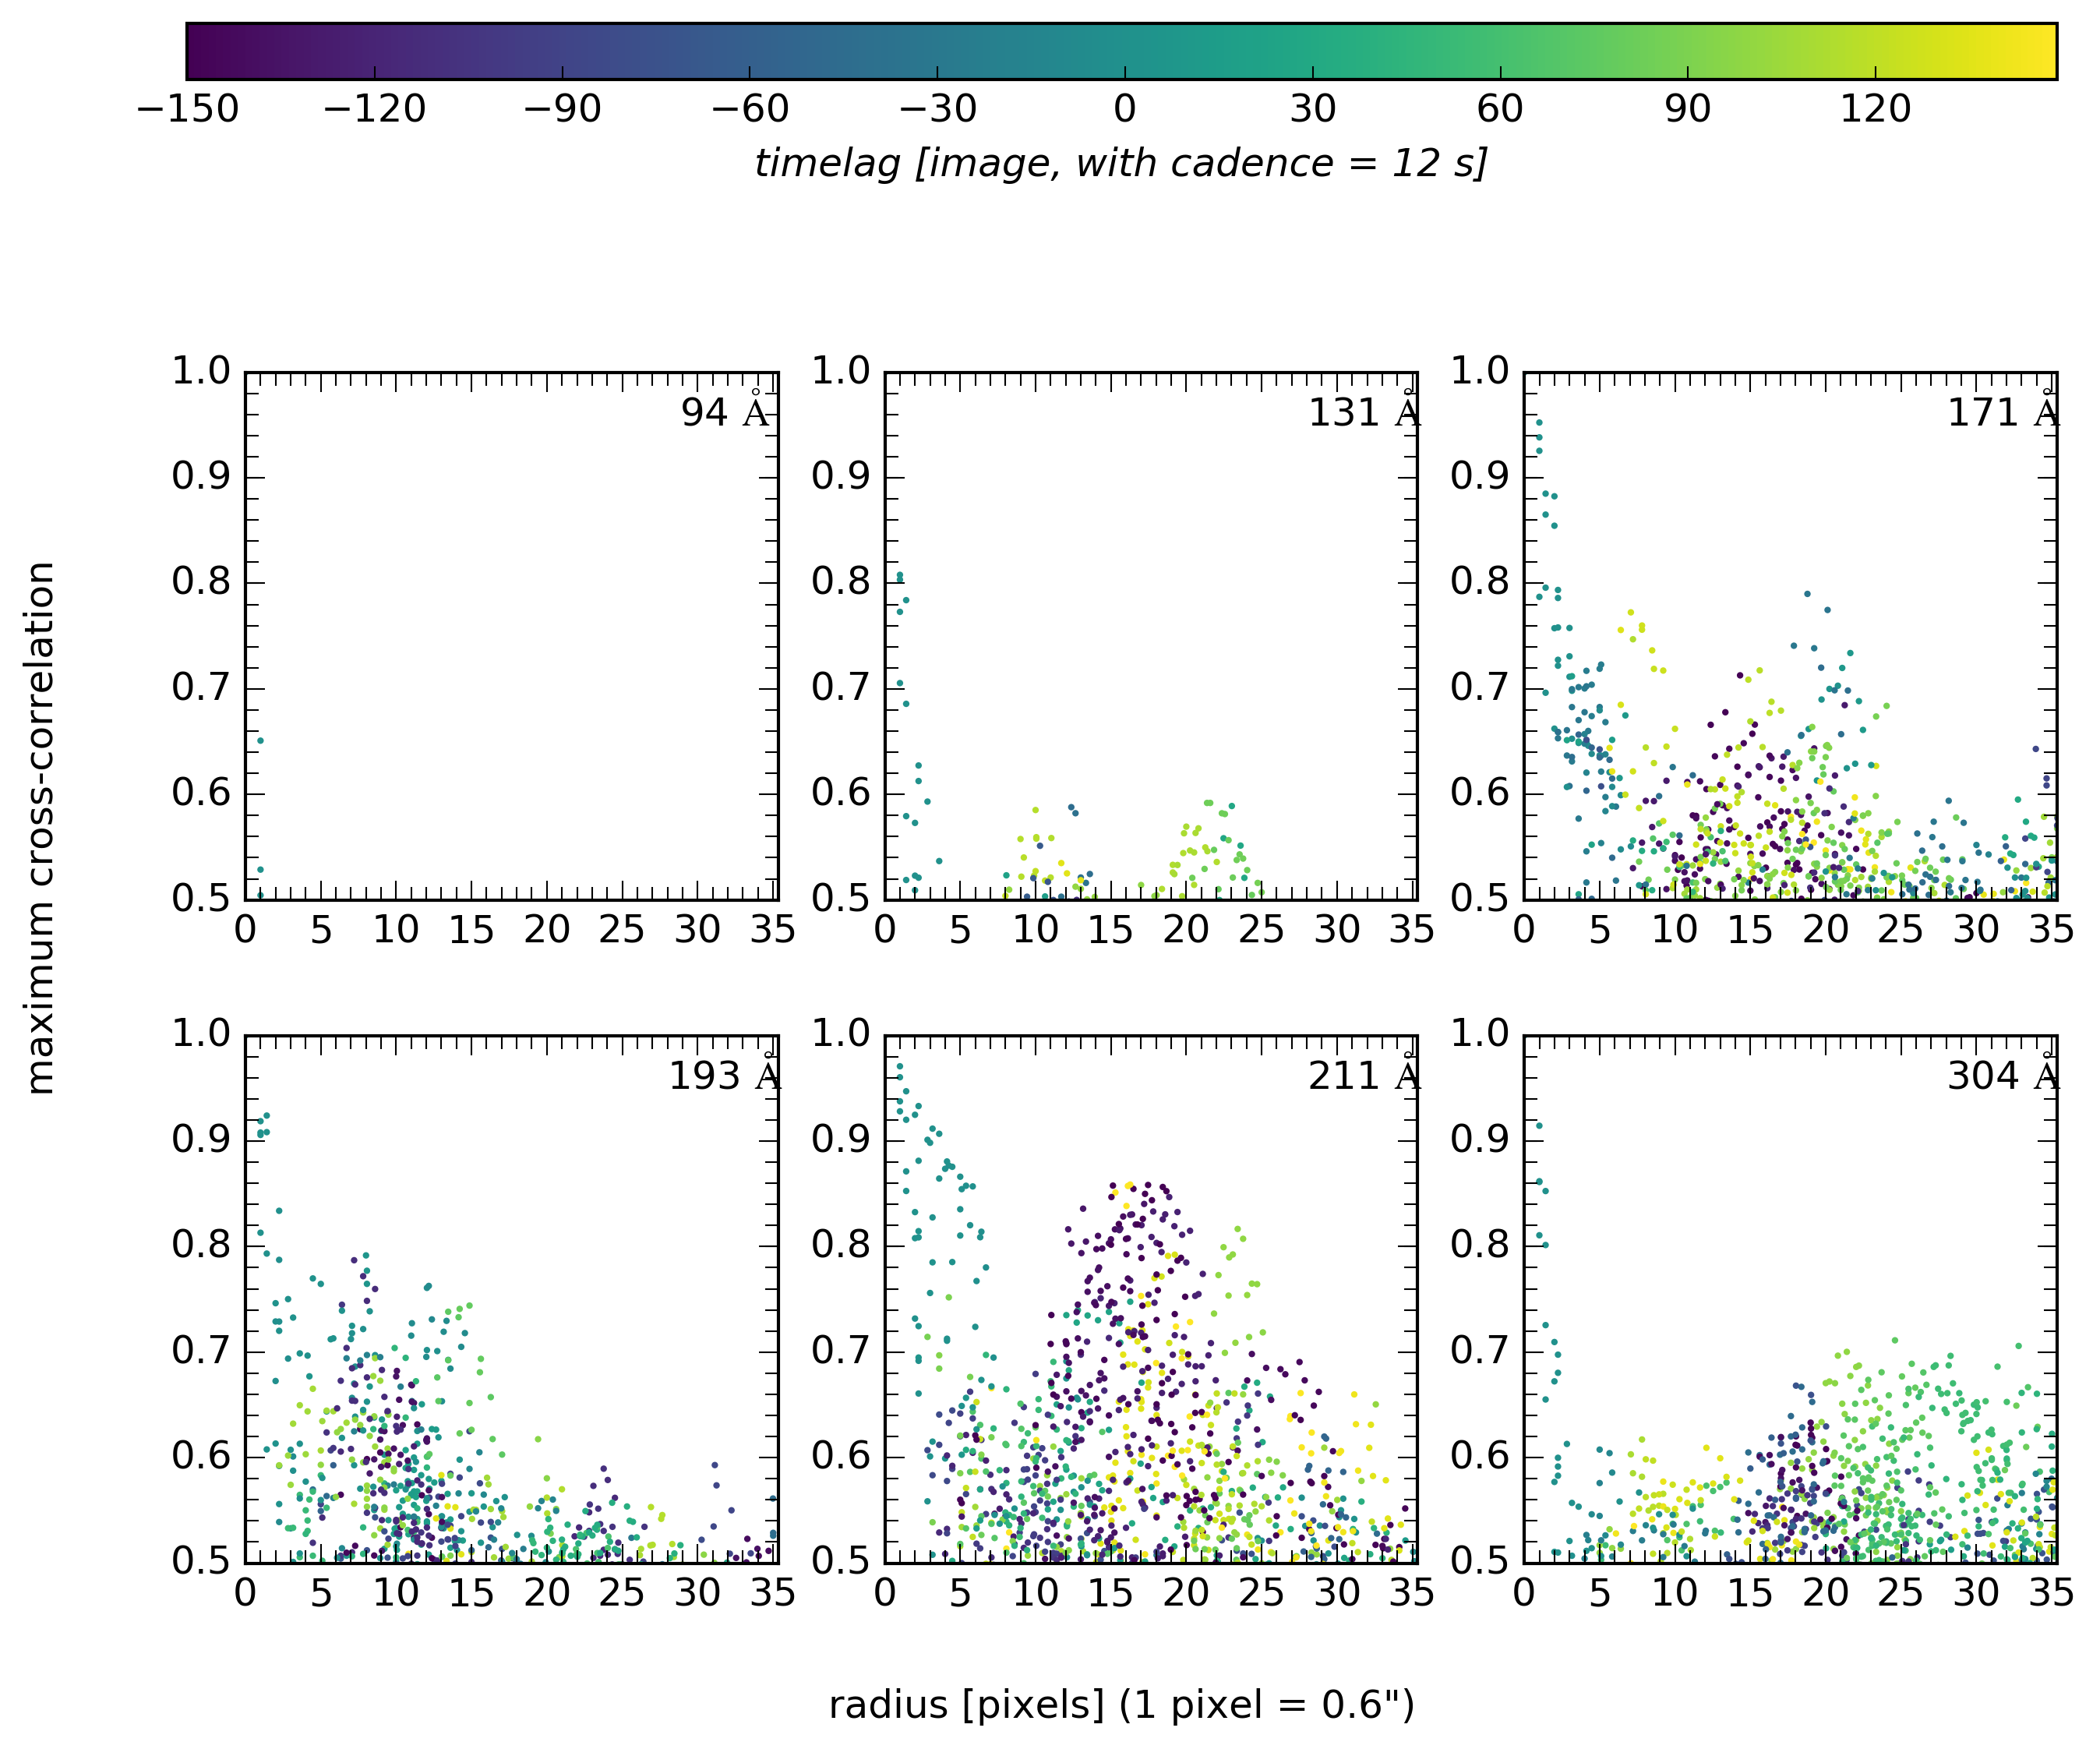
\includegraphics[width=\textwidth]{figure_4.png}
    \caption{The highest cross-correlation value of each pixel is plotted against
        its distance from the center pixel. The color indicates the timelag at which
        the highest cross-correlation occurred.}
    \label{tau_all}
\end{figure*}

\begin{figure*}[htb!]
    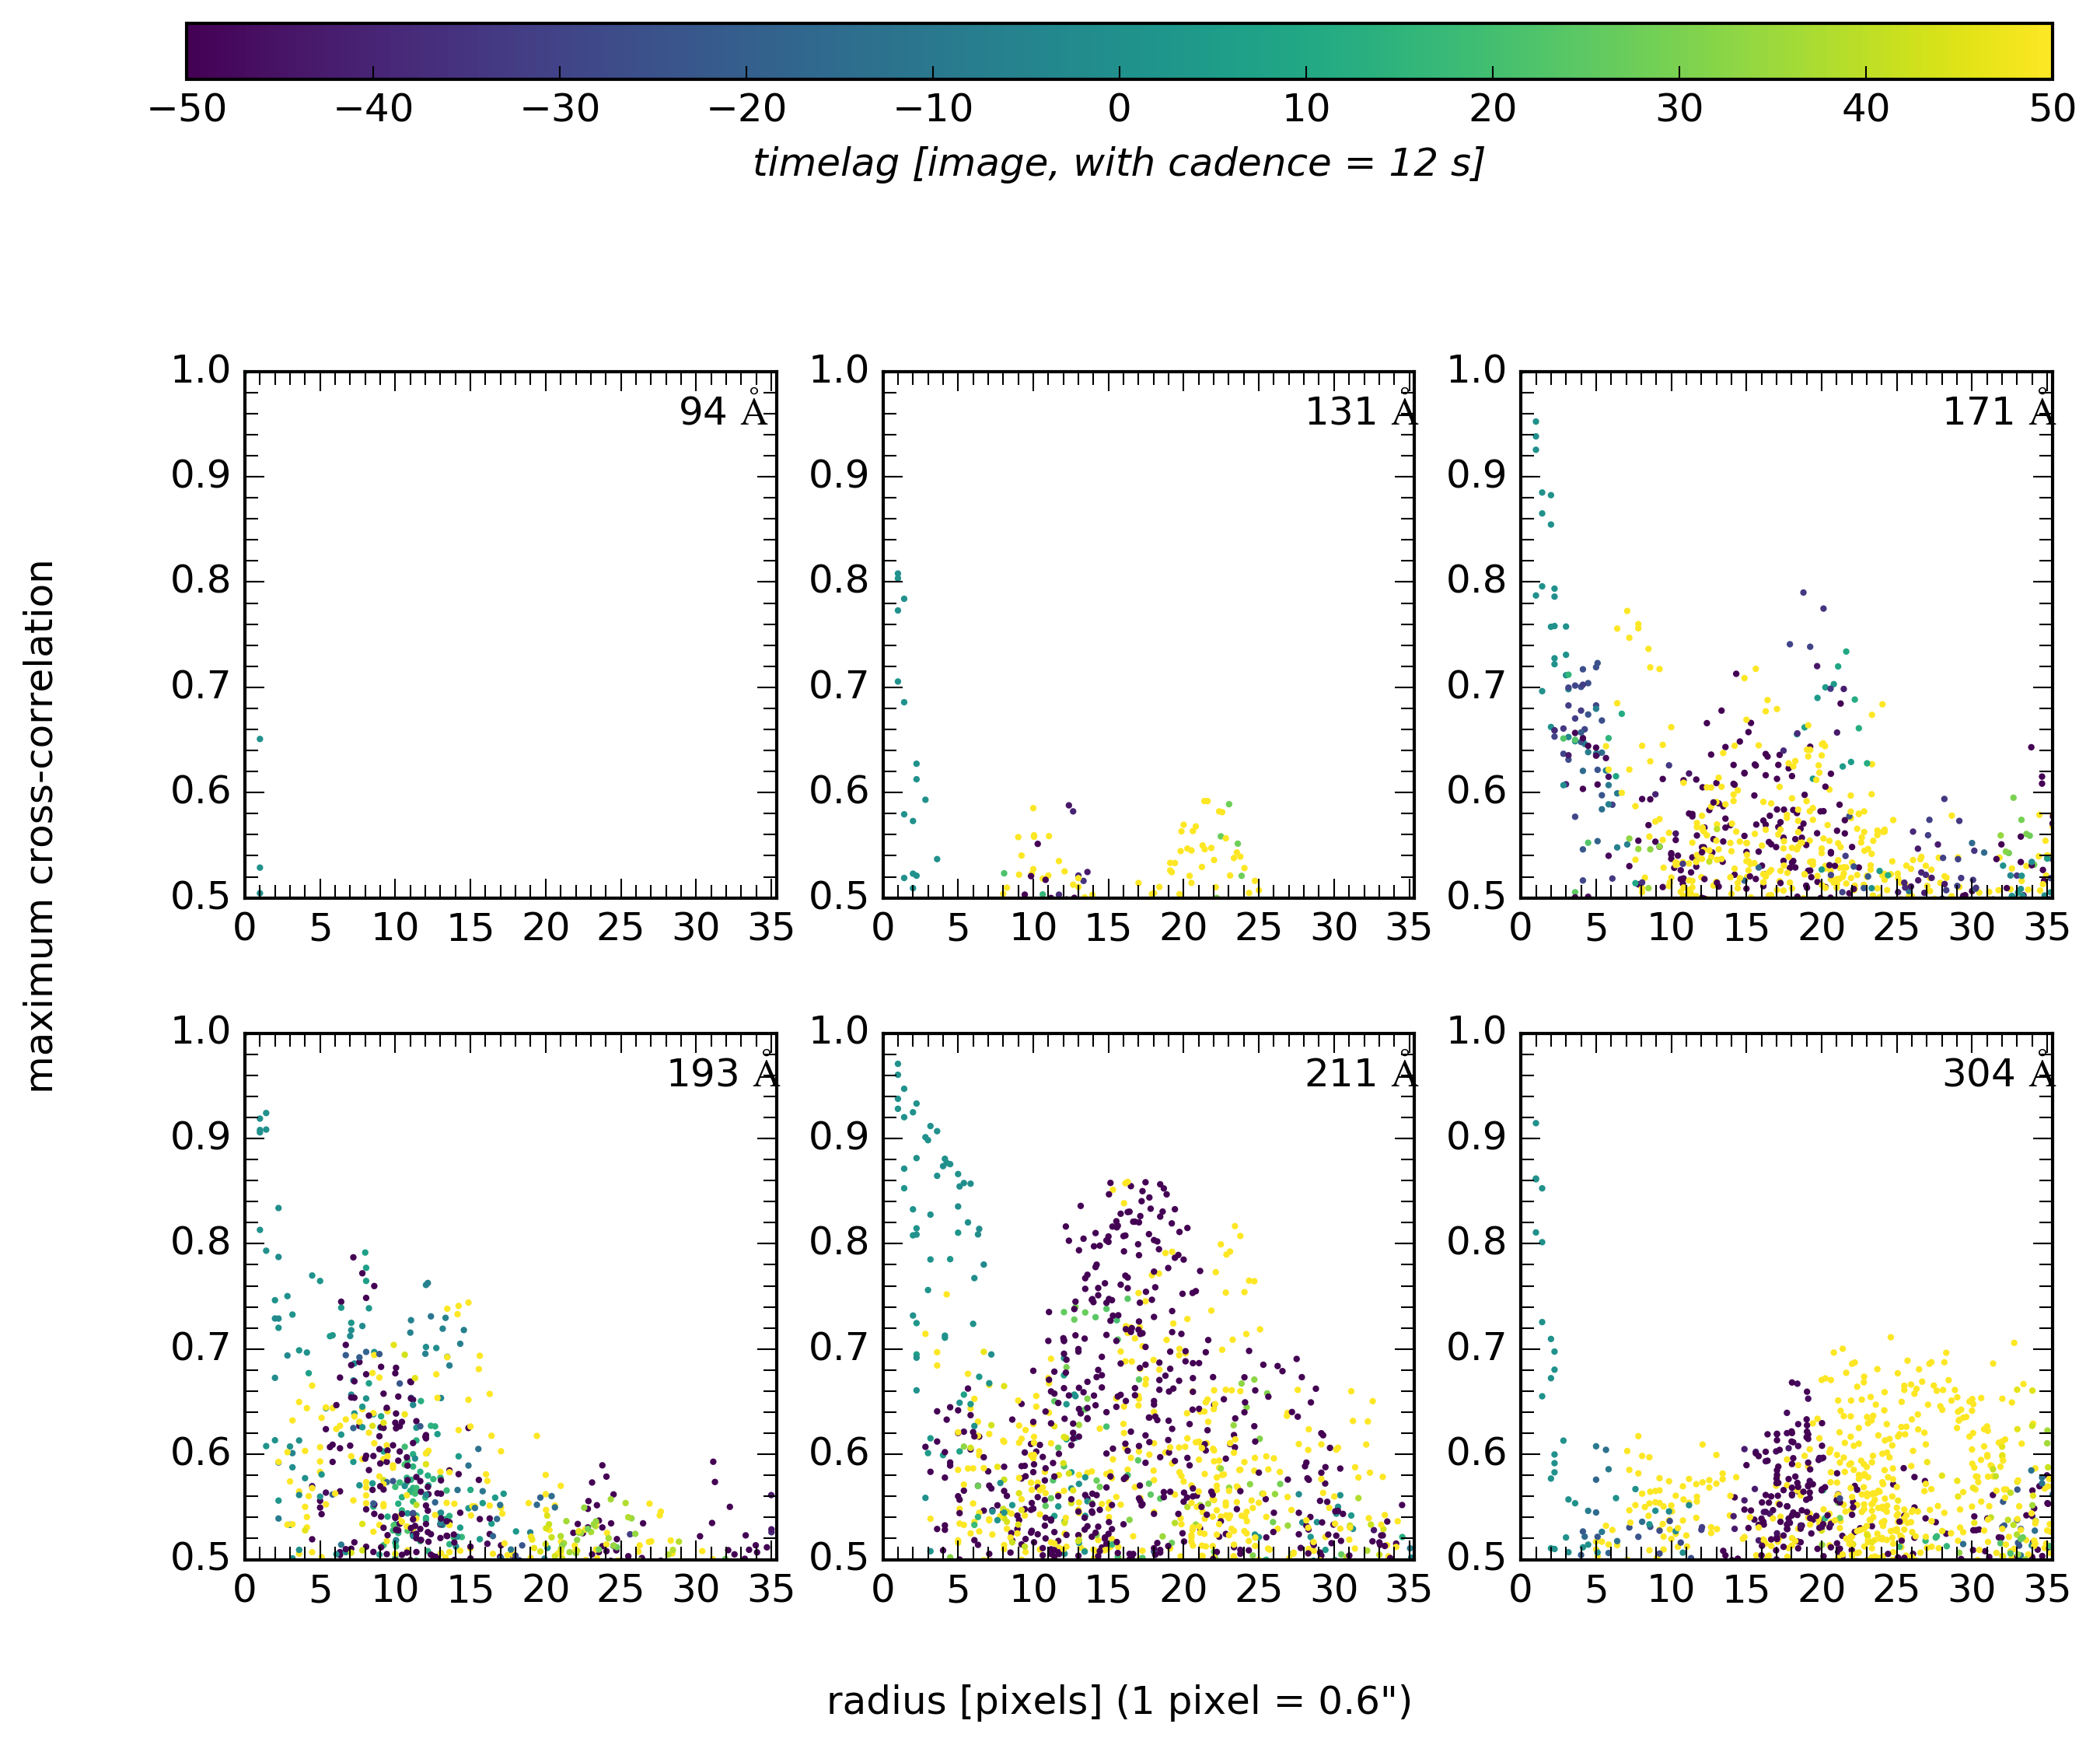
\includegraphics[width=\textwidth]{figure_5.png}
    \caption{Same as figure \ref{tau_all}, but with two thirds of the timelag cut out.}
\end{figure*}

\section{Analysis}\label{analysis}
The intensity of each BP as a function of radius gives a rough visual estimate
of the size of the BP. Here the estimate was taken a step further, using the
cross-correlation of the BP pixels through the entire time series.

\section{Results}\label{results}
\section{Conclusion}\label{conclusion}

\bibliography{reffile}
\end{document}
